\documentclass{article}
\usepackage{xeCJK}
\title{Robotics Homework 1}
  \author{龙肖灵 \\Xiaoling Long\\Student ID.: 81943968\\email:longxl@shanghaitech.edu.cn}
%\usepackage[utf8]{inputenc}
\usepackage{graphicx}
\usepackage[colorlinks,linkcolor=red]{hyperref}
  \DeclareGraphicsExtensions{.png,.pdf}
\usepackage{amsmath, amsthm, amssymb}
%\usepackage{subfloat}
\newtheorem{prop}{Proposition}
\usepackage{ulem}
\usepackage{indentfirst}
\begin{document}
\maketitle
\begin{description}
  \item[1.Prepare Ubuntu:] Done.
  \item[2.Install ROS:]
  Figure 1 is my screenshoot after I finished this work.
  \begin{figure}[h]
    \centering
    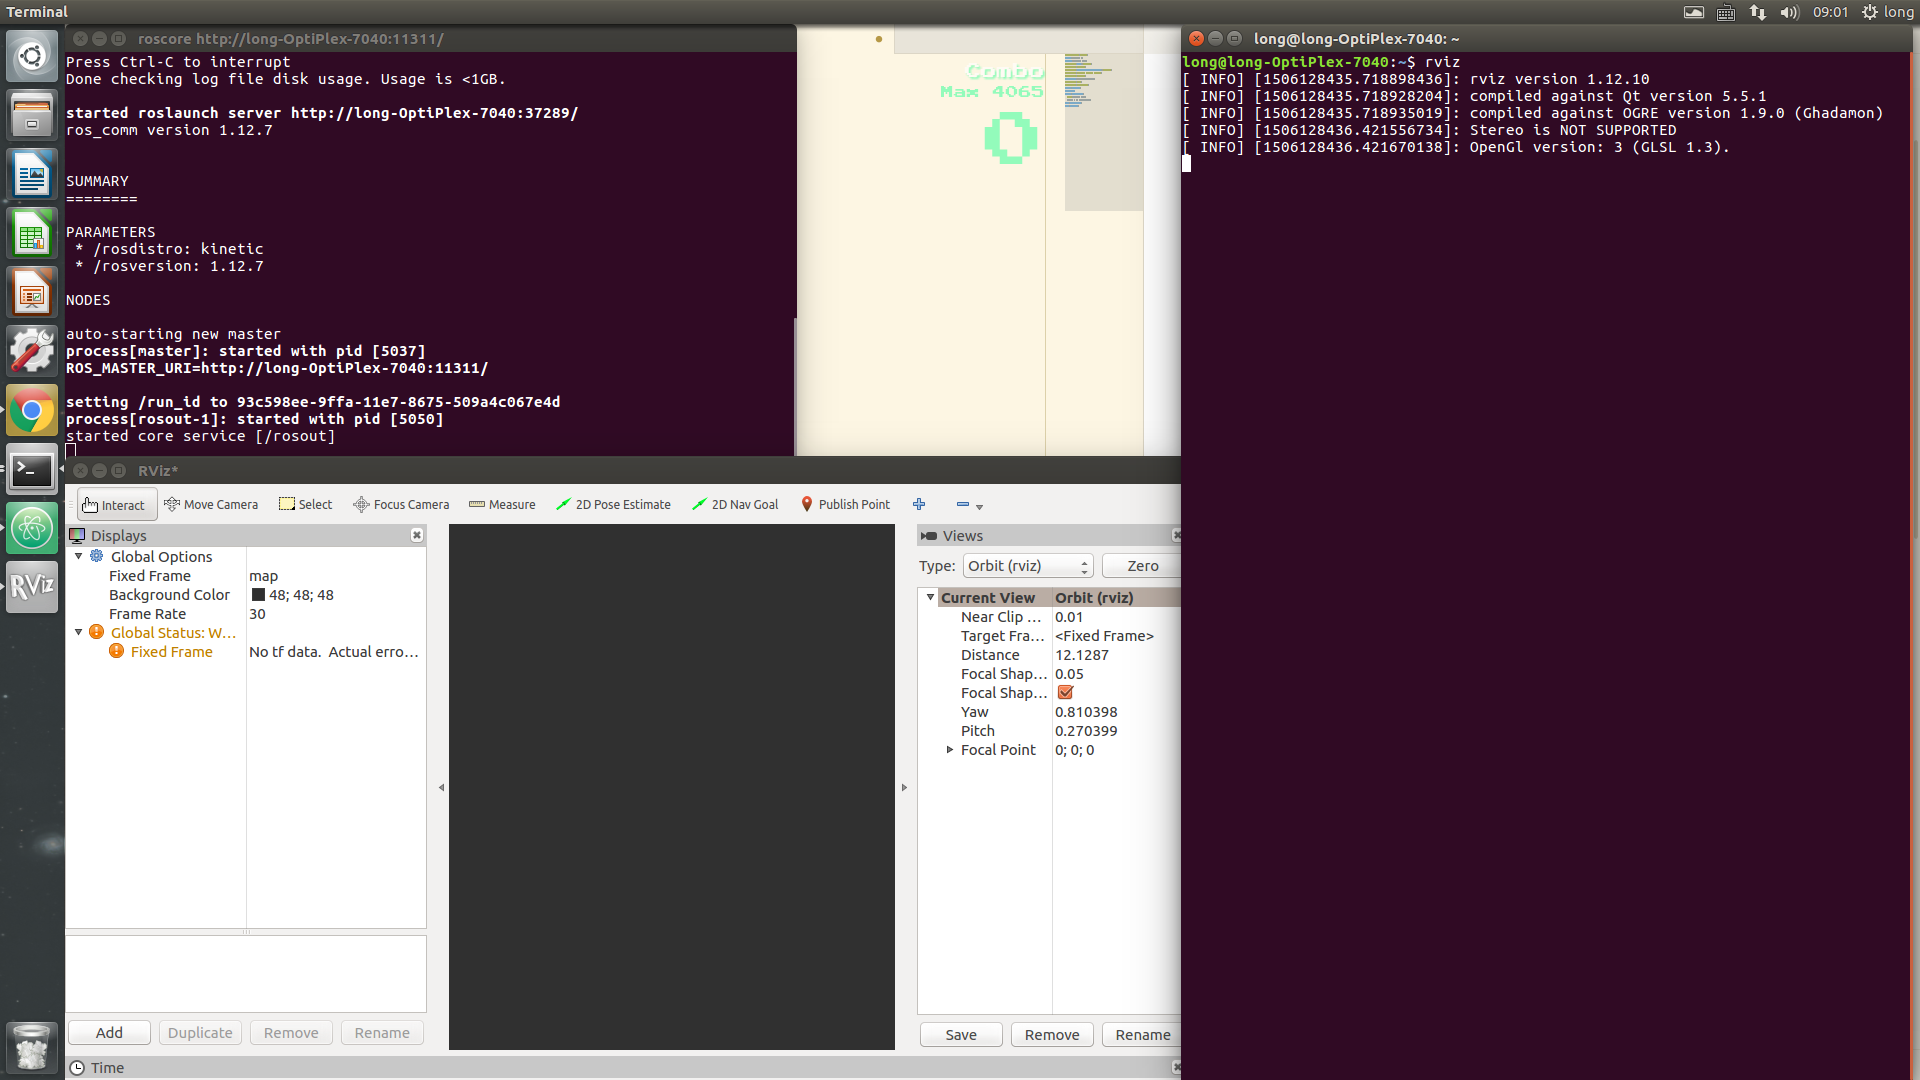
\includegraphics[width=\textwidth]{hw1.png}
    \caption{A screenshoot after finishing installing.}
    \label{fig:mesh1}
   \end{figure}
   \item[3.Shakey the Robot:]There is three questions.
   \begin{enumerate}
     \item I found the quantitative properties as following and compared to my cell phone.
    \begin{center}
       \begin{tabular}{|c | c | c|}
       \hline
       CPU Speed & $20 Mhz$(I guess) & $1.8Ghz$($200$ times) \\
       \hline
       RAM & $256 kB$(Computed) & $2GB$(too much) \\
       \hline
       Size & $1 \times1 \times1 (m^3)$(Guess) & $138\times 67\times 6.9(mm^3)$\\
       \hline
       Words Lenth & $36 bit$(Searched online) & $64bit$(twice)\\
       \hline
       Cam Resolution & $256\times 256$(Guess too) & about $1.2\times 10^8$(emm)\\ [1ex]
       \hline
      \end{tabular}
    \end{center}
    \item Compare to my cell phone, I think these values are so little. But shakey can still
    finish these amazing work based on these hardware. This is a amazing work. And a big step
    in the history of robotics.
    \item First step, Shakey takes a picture on object, and then extracts the lines from the
    picture of object. After that compares it with picture in library stored before. Finally
    he can recongnize the object if in library.
   \end{enumerate}
   \item[4 GIT:] I have sent my public key to TA. And can see my repo after ssh operation.
\end{description}
\end{document}
